\documentclass[11pt,oneside]{article}

\usepackage[utf8]{inputenc}
\usepackage[T1]{fontenc}
\usepackage[spanish,es-tabla]{babel}
\usepackage{lmodern}
\usepackage{microtype}
\usepackage[a4paper,top=1.85cm,bottom=2.05cm,left=1.85cm,right=1.85cm,headheight=24pt]{geometry}
\usepackage[table]{xcolor}
\usepackage{tikz}
\usetikzlibrary{calc,positioning,arrows.meta,shadows.blur}
\usepackage{booktabs}
\usepackage{longtable}
\usepackage{tabularx}
\usepackage{array}
\usepackage{enumitem}
\usepackage{titlesec}
\usepackage{fancyhdr}
\usepackage{hyperref}
\usepackage{graphicx}
\usepackage{caption}
\usepackage{amsmath}
\usepackage{float}

% -----------------------------------------------------------------------------
% Paleta visual Don Gato: alineada con el frontend.
% -----------------------------------------------------------------------------
\definecolor{coffeeBg}{HTML}{965640}
\definecolor{coffeeDeep}{HTML}{713825}
\definecolor{coffeePanel}{HTML}{EFE3C8}
\definecolor{coffeePanelLight}{HTML}{F8EED8}
\definecolor{coffeeInk}{HTML}{21140F}
\definecolor{coffeeMute}{HTML}{7A6858}
\definecolor{coffeeButton}{HTML}{AD6046}
\definecolor{inputBlue}{HTML}{EAF0FF}
\definecolor{deepNavy}{HTML}{0B1320}
\definecolor{panel}{HTML}{F7F9FC}
\definecolor{tealDark}{HTML}{0E6B6F}
\definecolor{leaf}{HTML}{6DAA3F}
\definecolor{gold}{HTML}{F0B84A}
\definecolor{coral}{HTML}{E35D5B}
\definecolor{violet}{HTML}{6B5DD3}

\hypersetup{
  colorlinks=true,
  linkcolor=coffeeDeep,
  urlcolor=tealDark,
  pdftitle={Informe Final Parcial I - Don Gato Inventory},
  pdfauthor={Equipo de trabajo ESPE}
}

\setlength{\parindent}{0pt}
\setlength{\parskip}{4.5pt}
\setlength{\textfloatsep}{8pt plus 2pt minus 2pt}
\setlength{\floatsep}{8pt plus 2pt minus 2pt}
\setlength{\intextsep}{8pt plus 2pt minus 2pt}
\setlist[itemize]{leftmargin=*,topsep=2pt,itemsep=1.5pt}
\setlist[enumerate]{leftmargin=*,topsep=2pt,itemsep=1.5pt}
\renewcommand{\arraystretch}{1.13}
\setcounter{tocdepth}{2}
\raggedbottom
\newcolumntype{Y}{>{\raggedright\arraybackslash}X}
\captionsetup{font=small,labelfont=bf,skip=4pt}
\arrayrulecolor{coffeeButton!45}
\graphicspath{{capturas/}}

% -----------------------------------------------------------------------------
% Encabezados y estilo editorial para secciones mayores.
% -----------------------------------------------------------------------------
\pagestyle{fancy}
\fancyhf{}
\lhead{\textcolor{coffeeDeep}{\textbf{Don Gato Inventory}}}
\rhead{\textcolor{deepNavy}{Informe Final Parcial I}}
\cfoot{\thepage}
\renewcommand{\headrulewidth}{0.4pt}
\renewcommand{\headrule}{\hbox to\headwidth{\color{coffeeButton}\leaders\hrule height \headrulewidth\hfill}}

\titleformat{\section}
  {\normalfont\LARGE\bfseries\color{coffeeInk}}
  {\tikz[baseline=(n.base)]\node[fill=coffeeButton,text=white,rounded corners=5pt,inner xsep=8pt,inner ysep=4pt,font=\large\bfseries](n){\thesection};}
  {0.7em}
  {}

\titleformat{\subsection}
  {\normalfont\Large\bfseries\color{coffeeDeep}}
  {\thesubsection}{0.6em}{}

\titleformat{\subsubsection}
  {\normalfont\normalsize\bfseries\color{deepNavy}}
  {\thesubsubsection}{0.5em}{}

\titlespacing*{\section}{0pt}{1.0em}{0.35em}
\titlespacing*{\subsection}{0pt}{0.8em}{0.25em}
\titlespacing*{\subsubsection}{0pt}{0.55em}{0.15em}

\newcommand{\chip}[2]{\tikz[baseline=(x.base)]\node[rounded corners=4pt,fill=#1!14,draw=#1!55,text=deepNavy,inner xsep=5pt,inner ysep=2pt,font=\scriptsize\bfseries](x){#2};}

\begin{document}

% -----------------------------------------------------------------------------
% Portada reutilizada: misma tematica visual del frontend.
% -----------------------------------------------------------------------------
\hypersetup{pageanchor=false}
\begin{titlepage}
\begin{tikzpicture}[remember picture,overlay]
  \fill[coffeeBg] (current page.south west) rectangle (current page.north east);
  \fill[coffeeDeep] (current page.north west) rectangle ([yshift=-1.55cm]current page.north east);
  \fill[coffeeDeep,opacity=.28] ([yshift=-1.55cm]current page.north west) rectangle (current page.south east);

  \foreach \x/\y/\r/\o in {1.2/-4.0/1.8/.08,18.8/-4.7/2.2/.07,2.0/-20.4/2.8/.06,18.0/-25.0/3.0/.08,10.5/-16.5/5.6/.05} {
    \fill[coffeePanelLight,opacity=\o] ([xshift=\x cm,yshift=\y cm]current page.north west) circle (\r cm);
  }

  \node[anchor=west,font=\bfseries\large,text=coffeePanelLight] at ([xshift=1.35cm,yshift=-.78cm]current page.north west) {Don Gato - Inventario};
  \node[anchor=east,font=\scriptsize,text=coffeePanelLight!78] at ([xshift=-1.35cm,yshift=-.78cm]current page.north east) {Informe Final Parcial I \, | \, SQA};

  \node[
    fill=coffeePanel,
    draw=coffeePanelLight!70,
    line width=.7pt,
    rounded corners=18pt,
    blur shadow={shadow xshift=0pt,shadow yshift=-5pt,shadow blur steps=8,shadow blur radius=8pt,shadow opacity=.35},
    minimum width=13.2cm,
    minimum height=22.7cm,
    anchor=center
  ] (card) at ([yshift=-.65cm]current page.center) {};

  % Emblema Don Gato tomado del frontend.
  \begin{scope}[shift={([yshift=8.35cm]card.center)}]
    \fill[coffeeInk] (0,0) circle (1.25);
    \fill[coffeePanelLight] (0,0) circle (1.14);
    \begin{scope}
      \clip (0,0) circle (1.03);
      \node at (0,0) {
\includegraphics[width=2.14cm,height=2.14cm]{portada-gato-don-gato.png}};
    \end{scope}
    \draw[coffeeInk,line width=1.05pt] (0,0) circle (1.04);
    \draw[coffeeButton,line width=1.35pt] (0,0) circle (1.24);
    \draw[coffeePanelLight,line width=.5pt,opacity=.8] (0,0) circle (1.11);
  \end{scope}

  \node[font=\bfseries\Huge,text=coffeeInk,align=center] at ([yshift=6.25cm]card.center) {Informe Final};
  \node[font=\bfseries\Large,text=coffeeInk,align=center] at ([yshift=5.45cm]card.center) {API REST Empresarial};
  \node[font=\large,text=coffeeMute,align=center,text width=10.4cm] at ([yshift=4.55cm]card.center)
    {Integracion de Spring Boot, Clean Architecture y DevSecOps bajo el Modelo de Calidad de McCall};

  \node[font=\bfseries\large,text=coffeeDeep,align=center,text width=10.8cm] at ([yshift=2.95cm]card.center)
    {UNIVERSIDAD DE LAS FUERZAS ARMADAS ESPE};
  \node[font=\normalsize,text=coffeeInk,align=center,text width=10.8cm] at ([yshift=2.05cm]card.center)
    {Departamento de Ciencias de la Computacion\\Aseguramiento de la Calidad de Software};

  \node[font=\bfseries\LARGE,text=coffeeButton,align=center,text width=11cm] at ([yshift=.55cm]card.center)
    {Cafeteria Don Gato\\Sistema de Gestion de Inventario};

  \node[rounded corners=6pt,fill=inputBlue,draw=coffeePanelLight!30,minimum width=10.8cm,minimum height=1.15cm] at ([yshift=-1.25cm]card.center) {};
  \node[font=\small,text=coffeeInk,align=center,text width=10.3cm] at ([yshift=-1.25cm]card.center)
    {\textbf{Docente:} Ing. Diego L. Gamboa\\[-1pt]\texttt{dlgamboa1@espe.edu.ec} \quad | \quad \textbf{Fecha:} 13 de mayo de 2026};

  \node[font=\bfseries,text=coffeeInk] at ([yshift=-2.70cm]card.center) {Equipo de trabajo};
  \node[font=\normalsize,text=coffeeInk,align=center,text width=10cm] at ([yshift=-3.55cm]card.center)
    {Mesias Mariscal \quad Gabriel Murillo\\Denise Rea \quad Julio Viche};

  \node[font=\small,text=coffeeMute,align=center] at ([yshift=-5.05cm]card.center)
    {\chip{coffeeButton}{Spring Boot 4.0.6} \quad \chip{tealDark}{17 endpoints} \quad \chip{leaf}{146 tests OK} \quad \chip{violet}{JWT + McCall}};

  \node[font=\scriptsize,text=coffeeMute,align=center,text width=10.6cm] at ([yshift=-6.35cm]card.center)
    {Documento final basado en PDCA, Modelo de McCall, Clean Architecture, pruebas automatizadas, cobertura JaCoCo, Quality Scoring Engine y evidencias DevSecOps.};
\end{tikzpicture}
\end{titlepage}

\clearpage
\hypersetup{pageanchor=true}
\pagenumbering{roman}
\tableofcontents
\clearpage
\pagenumbering{arabic}

% -----------------------------------------------------------------------------
\section{Introduccion}

\subsection{Contexto del Problema}

La cafeteria Don Gato requiere controlar productos, categorias y movimientos de inventario de forma segura, trazable y consistente. En este tipo de proceso, una salida mal registrada, una categoria duplicada o un producto actualizado sin control puede afectar la disponibilidad del negocio, producir compras innecesarias y disminuir la confiabilidad de la informacion operativa.

El proyecto atiende esta necesidad mediante una API REST versionada para la gestion de inventario. La solucion separa las consultas publicas, necesarias para el frontend, de las operaciones administrativas protegidas por autenticacion JWT. Esta decision permite que el sistema mantenga una experiencia de usuario sencilla sin renunciar a controles de integridad para las acciones sensibles.

\subsection{Objetivos}

El objetivo general es construir una API REST empresarial educativa para la gestion de inventario de la cafeteria Don Gato, aplicando principios de Clean Architecture, seguridad JWT, pruebas automatizadas y evaluacion de calidad bajo el Modelo de McCall.

Los objetivos especificos son:

\begin{itemize}
  \item implementar los modulos de autenticacion, categorias, productos y movimientos de stock;
  \item separar dominio, aplicacion, infraestructura e interfaces para mejorar mantenibilidad y testabilidad;
  \item proteger operaciones administrativas mediante tokens JWT;
  \item validar el backend con pruebas automatizadas y cobertura JaCoCo;
  \item consolidar resultados de calidad mediante un Quality Scoring Engine;
  \item relacionar las decisiones tecnicas con el ciclo PDCA y los factores de McCall.
\end{itemize}

\subsection{Alcance del MVP}

El MVP cubre las funciones necesarias para operar el inventario base de la cafeteria. No busca resolver todos los escenarios comerciales futuros, sino entregar una base tecnicamente solida que pueda crecer hacia roles, reportes, analitica y documentacion viva de API.

\begin{table}[H]
\centering
\small
\caption{Alcance funcional del MVP}
\begin{tabularx}{\textwidth}{>{\bfseries}p{.27\textwidth}Y}
\toprule
Modulo & Alcance implementado\\
\midrule
Autenticacion & Inicio de sesion con JWT y respuesta tipo Bearer.\\
Categorias & Creacion, listado, busqueda por id, actualizacion y eliminacion.\\
Productos & Creacion, listado, busqueda por id, filtrado por categoria, filtrado por estado, busqueda por nombre, actualizacion y eliminacion.\\
Movimientos de stock & Registro de entradas y salidas, listado general y consulta por producto.\\
Seguridad & Consultas publicas para productos y categorias; escritura y movimientos protegidos por JWT.\\
Calidad & Pruebas con JUnit, Mockito, H2 y Spring Security Test; cobertura JaCoCo; configuracion OWASP y JMeter.\\
\bottomrule
\end{tabularx}
\end{table}

La calidad se considero desde el diseno. Las reglas de negocio se aislaron en el dominio, los casos de uso se hicieron testeables, la API se versiono bajo \texttt{/api/v1}, la seguridad se configuro por rutas y las metricas se conectaron con el Quality Score.

% -----------------------------------------------------------------------------
\section{Metodologia}

\subsection{Aplicacion del Ciclo PDCA}

El desarrollo se organizo con el ciclo \textbf{Plan-Do-Check-Act}. En la fase de planificacion se definieron el problema, el alcance y los criterios de calidad. En la fase de ejecucion se implementaron las capas del sistema y los controles de seguridad. En la fase de verificacion se ejecutaron pruebas y metricas. En la fase de actuacion se identificaron mejoras necesarias para fortalecer el proceso DevSecOps.

\begin{figure}[H]
\centering
\begin{tikzpicture}[
  stage/.style={circle,draw=coffeeButton,fill=coffeePanelLight,line width=.7pt,minimum size=2.65cm,align=center,font=\bfseries\small,text=coffeeInk},
  arr/.style={-{Latex[length=3mm]},thick,coffeeButton}
]
  \node[stage] (plan) at (90:3.0cm) {PLAN\\\footnotesize alcance\\calidad};
  \node[stage] (do) at (0:3.0cm) {DO\\\footnotesize backend\\seguridad};
  \node[stage] (check) at (-90:3.0cm) {CHECK\\\footnotesize pruebas\\metricas};
  \node[stage] (act) at (180:3.0cm) {ACT\\\footnotesize mejora\\continua};
  \node[align=center,font=\bfseries\small,text=coffeeDeep] at (0,0) {Don Gato\\Inventory};
  \draw[arr,bend left=15] (plan) to (do);
  \draw[arr,bend left=15] (do) to (check);
  \draw[arr,bend left=15] (check) to (act);
  \draw[arr,bend left=15] (act) to (plan);
\end{tikzpicture}
\caption{Ciclo PDCA aplicado al proyecto}
\end{figure}

\subsection{Modelo de McCall}

El Modelo de McCall se uso como marco de evaluacion porque permite relacionar requisitos tecnicos con atributos de calidad. En este proyecto se priorizaron Correctness, Reliability, Integrity, Maintainability, Testability, Portability e Interoperability.

\begin{table}[H]
\centering
\small
\caption{Factores de McCall aplicados al proyecto}
\begin{tabularx}{\textwidth}{>{\bfseries}p{.25\textwidth}p{.34\textwidth}Y}
\toprule
Perspectiva & Factores & Aplicacion en Don Gato Inventory\\
\midrule
Operacion del producto & Correctness, Reliability, Efficiency, Integrity, Usability & Reglas de stock, respuestas HTTP, JWT, validaciones y experiencia del frontend.\\
Revision del producto & Maintainability, Flexibility, Testability & Clean Architecture, puertos, DTOs, mappers y pruebas automatizadas.\\
Transicion del producto & Portability, Reusability, Interoperability & Maven Wrapper, Docker, PostgreSQL y API REST versionada.\\
\bottomrule
\end{tabularx}
\end{table}

\subsection{Trazabilidad entre Requisitos y Calidad}

\begin{table}[H]
\centering
\small
\caption{Mapeo de requisitos a factores de McCall}
\begin{tabularx}{\textwidth}{p{.22\textwidth}p{.17\textwidth}p{.27\textwidth}Y}
\toprule
Requisito & Factor & Metrica & Validacion\\
\midrule
Autenticacion JWT & Integrity & Rutas protegidas & Spring Security y pruebas de acceso.\\
Reglas de stock & Correctness & Cero defectos funcionales en pruebas & JUnit y Mockito.\\
Cobertura alta & Testability & Mayor o igual a 85\% & JaCoCo.\\
Arquitectura limpia & Maintainability & Separacion de capas & Revision de estructura.\\
Despliegue reproducible & Portability & Entorno ejecutable por configuracion & Maven Wrapper y Docker.\\
API versionada & Interoperability & 17 endpoints REST & Controladores bajo \texttt{/api/v1}.\\
Rendimiento base & Efficiency & Objetivo menor a 200 ms & Plan JMeter.\\
\bottomrule
\end{tabularx}
\end{table}

\subsection{Clean Architecture}

La arquitectura separa el dominio de los detalles externos. Esta decision reduce acoplamiento y permite que las reglas del inventario puedan probarse sin depender de controladores HTTP, entidades JPA o configuracion de seguridad.

\begin{figure}[H]
\centering
\begin{tikzpicture}[
  layer/.style={draw=coffeeButton,rounded corners=5pt,minimum width=12.2cm,minimum height=.9cm,align=center,font=\bfseries\small},
  note/.style={font=\scriptsize,text=coffeeMute}
]
  \node[layer,fill=coffeePanelLight] (domain) at (0,0) {Dominio: modelos, reglas de negocio y excepciones};
  \node[layer,fill=panel,below=.20cm of domain] (app) {Aplicacion: casos de uso y puertos};
  \node[layer,fill=inputBlue,below=.20cm of app] (infra) {Infraestructura: JPA, PostgreSQL, adapters, seguridad y configuracion};
  \node[layer,fill=coffeePanel,below=.20cm of infra] (api) {Interfaces: controladores REST, DTOs, mappers y manejo de errores};
  \draw[-{Latex[length=2.5mm]},thick,coffeeDeep] ([xshift=-5.6cm]api.north) -- ([xshift=-5.6cm]domain.south);
  \node[note,rotate=90] at (-6.0,-1.55) {dependencias hacia el dominio};
\end{tikzpicture}
\caption{Separacion de capas usada en el backend}
\end{figure}

\subsection{Matriz PDCA de Seguimiento}

La hoja de calculo del equipo, identificada como \textit{PROYECTO INVENTARIO}, se utiliza como evidencia de gestion del ciclo PDCA. Su informacion es compatible con el informe porque registra objetivo, responsables, avance, metricas y actividades por etapa. Para evitar duplicacion, el documento conserva solo los datos necesarios para demostrar trazabilidad.

\begin{table}[H]
\centering
\small
\caption{Datos principales de la matriz PDCA}
\begin{tabularx}{\textwidth}{>{\bfseries}p{.22\textwidth}Y}
\toprule
Elemento & Registro principal\\
\midrule
Proyecto & Inventario Don Gato - SQA.\\
Proceso & Arquitectura Hexagonal y SQA basado en McCall.\\
Ciclo & Ciclo 1.\\
Objetivo & Backend empresarial con arquitectura hexagonal, 17 endpoints validados, seguridad JWT y puntaje McCall superior a 80/100.\\
Metricas & Cobertura JaCoCo, latencia JMeter, vulnerabilidades OWASP y Quality Score.\\
\bottomrule
\end{tabularx}
\end{table}

\begin{table}[H]
\centering
\small
\caption{Avance por etapa PDCA registrado por el equipo}
\begin{tabularx}{\textwidth}{p{.17\textwidth}Yp{.18\textwidth}p{.12\textwidth}}
\toprule
Etapa & Actividades registradas & Responsable & Avance\\
\midrule
Planificar & Requerimientos, diseno arquitectonico, factores McCall y plan de pruebas. & Dev / QA & 100\%\\
Hacer & Dominio, infraestructura, PostgreSQL, Docker, seguridad JWT y Quality Engine. & Dev & 100\%\\
Verificar & Pruebas unitarias, validacion de carga y auditoria OWASP. & QA / Dev & 100\%\\
Actuar & Quality gates, mejora de mantenibilidad, documentacion y cierre del ciclo. & Dev & 100\%\\
\bottomrule
\end{tabularx}
\end{table}

\subsection{Concordancia entre Matriz y Evidencia Tecnica}

La matriz PDCA documenta el seguimiento del proceso, mientras que los reportes generados por herramientas aportan la evidencia tecnica. Cuando aparece una diferencia menor entre un registro manual y un reporte automatizado, el informe utiliza el valor automatizado y conserva la matriz como respaldo de planificacion y control.

\begin{table}[H]
\centering
\small
\caption{Conciliacion de datos entre matriz e informe}
\begin{tabularx}{\textwidth}{p{.20\textwidth}p{.23\textwidth}Yp{.18\textwidth}}
\toprule
Indicador & Matriz PDCA & Evidencia usada en informe & Lectura\\
\midrule
Cobertura & 91.5\% & JaCoCo local: 90.77\% en lineas y 92\% en instrucciones; SonarCloud: 83.5\% en \textit{overall code}. & Cumple en JaCoCo; SonarCloud aprueba el Quality Gate.\\
Latencia & 185 ms & Plan JMeter orientado a validar respuestas menores a 200 ms. & Registro compatible.\\
Vulnerabilidades & 0 criticas & SonarCloud reporta Security Rating A; OWASP Dependency Check queda configurado como gate. & Sin issues de seguridad abiertos en SonarCloud.\\
Pipeline & CI/CD operativo & GitHub Actions registra 35 corridas de workflow y ejecuciones recientes exitosas. & Captura disponible.\\
SonarCloud & 23 issues iniciales & Resultado final: 0 open issues, 0.0\% duplicacion y Quality Gate aprobado. & Mejora verificada.\\
Avance PDCA & 100\% por etapa & Informe cerrado con resultados y acciones de mejora. & Coherente.\\
\bottomrule
\end{tabularx}
\end{table}

La diferencia entre 91.5\%, 90.77\% y 83.5\% no representa una contradiccion: corresponden a fuentes y alcances distintos. La matriz PDCA registra el seguimiento del equipo, JaCoCo mide la cobertura local del backend y SonarCloud calcula cobertura sobre \textit{overall code} con sus propias reglas de analisis. Para el calculo del Quality Score se utiliza 90.77\%, por ser el dato exacto disponible en el reporte JaCoCo local; para mantenibilidad se usa el estado final de SonarCloud con 0 open issues.

% -----------------------------------------------------------------------------
\section{Resultados}

\subsection{Metricas de Calidad Obtenidas}

La evidencia local fue generada el 13 de mayo de 2026 mediante la ejecucion de pruebas del backend. Los reportes de Surefire y JaCoCo indican que el proyecto cumple el umbral de cobertura establecido y no presenta fallos funcionales en la bateria automatizada disponible. Las capturas incorporadas despues de la mejora muestran tambien el estado de SonarCloud y GitHub Actions como evidencia visual del proceso DevSecOps.

\begin{table}[H]
\centering
\small
\caption{Resultados locales de pruebas y cobertura}
\begin{tabularx}{\textwidth}{p{.30\textwidth}Yp{.20\textwidth}}
\toprule
Area & Indicador & Resultado\\
\midrule
Pruebas automatizadas & Suites ejecutadas & 24\\
Pruebas automatizadas & Casos ejecutados & 146\\
Pruebas automatizadas & Fallos, errores y omitidas & 0 / 0 / 0\\
Cobertura JaCoCo & Instrucciones & 92\%\\
Cobertura JaCoCo & Ramas & 78\%\\
Cobertura JaCoCo & Lineas & 90.77\%\\
Cobertura JaCoCo & Metodos & 91.52\%\\
Cobertura JaCoCo & Clases & 90.63\%\\
\bottomrule
\end{tabularx}
\end{table}

\begin{table}[H]
\centering
\small
\caption{Indicadores de calidad y seguridad}
\begin{tabularx}{\textwidth}{>{\bfseries}p{.32\textwidth}Y}
\toprule
Indicador & Resultado\\
\midrule
Defectos en pruebas & No se registraron fallos ni errores en la ejecucion automatizada local.\\
SonarCloud Quality Gate & Estado \textit{Passed}; todas las condiciones del gate fueron aprobadas.\\
SonarCloud Open Issues & 0 issues abiertos en el analisis final; inicialmente existian 23 hallazgos de mantenibilidad.\\
SonarCloud Coverage & 83.5\% sobre \textit{overall code}; se reporta como lectura externa distinta de JaCoCo local.\\
SonarCloud Duplications & 0.0\% de duplicacion.\\
Vulnerabilidades criticas & El umbral definido es 0 criticas; SonarCloud muestra Security Rating A y OWASP Dependency Check queda configurado para el ciclo \texttt{verify}.\\
Endpoints activos & 17 endpoints REST versionados bajo \texttt{/api/v1}.\\
Seguridad & JWT para operaciones protegidas; consultas publicas controladas para productos y categorias.\\
Pipeline GitHub Actions & 35 corridas de workflow registradas y ejecuciones recientes en estado exitoso.\\
Rendimiento & La matriz registra 185 ms y el plan JMeter mantiene el objetivo menor a 200 ms.\\
\bottomrule
\end{tabularx}
\end{table}

\subsection{Quality Score Calculado}

El Quality Scoring Engine pondera cuatro factores de McCall: Testability, Correctness, Maintainability e Integrity. El calculo usa cobertura de lineas como medida de testabilidad, resultados de pruebas como medida de correctitud, los issues abiertos de SonarCloud como referencia de mantenibilidad y el criterio de cero vulnerabilidades criticas como integridad.

\[
Score = (Testability \times 0.30) + (Correctness \times 0.30) + (Maintainability \times 0.20) + (Integrity \times 0.20)
\]

\begin{table}[H]
\centering
\small
\caption{Calculo del Quality Score}
\begin{tabular}{lrrr}
\toprule
Factor & Valor & Peso & Aporte\\
\midrule
Testability & 90.77 & 0.30 & 27.23\\
Correctness & 100.00 & 0.30 & 30.00\\
Maintainability & 100.00 & 0.20 & 20.00\\
Integrity & 100.00 & 0.20 & 20.00\\
\midrule
\textbf{Total} & & & \textbf{97.23 / 100}\\
\bottomrule
\end{tabular}
\end{table}

El resultado de 97.23/100 ubica al MVP en un nivel alto para el alcance academico del proyecto. La mejora respecto al calculo anterior se explica por la correccion de hallazgos de mantenibilidad en SonarCloud, que paso de 23 issues abiertos a 0. Las mejoras pendientes se concentran en aumentar cobertura de ramas y publicar artefactos finales de OWASP y JMeter dentro del pipeline.

\subsection{Evidencias de Ejecucion}

Las evidencias se presentan de manera documental, asociando cada fuente con su resultado y con el factor McCall correspondiente. Este formato evita duplicar salidas de consola y mantiene el informe como documento formal.

\begin{table}[H]
\centering
\small
\caption{Evidencias tecnicas consolidadas}
\begin{tabularx}{\textwidth}{p{.24\textwidth}Yp{.22\textwidth}}
\toprule
Fuente & Resultado registrado & Factor McCall\\
\midrule
Surefire / Maven Test & 146 pruebas ejecutadas, sin fallos, errores ni casos omitidos. & Testability, Reliability\\
JaCoCo & Cobertura de lineas de 90.77\% y cobertura de instrucciones de 92\%. & Testability\\
SonarCloud inicial & 23 issues de mantenibilidad, con 19 de severidad media y 4 de severidad baja. & Maintainability\\
SonarCloud final & Quality Gate aprobado, 0 open issues, 0.0\% duplicacion, 83.5\% de cobertura overall code y Security Rating A. & Maintainability, Integrity\\
GitHub Actions & Workflow DevSecOps con 35 corridas registradas y ejecuciones recientes exitosas. & Portability, Reliability\\
Spring Security & Separacion entre rutas publicas y rutas protegidas con JWT. & Integrity\\
Matriz PDCA & Avance de 100\% en Planificar, Hacer, Verificar y Actuar. & Maintainability\\
JMeter & Registro de latencia de 185 ms en la matriz de seguimiento. & Efficiency\\
OWASP Dep. Check & Control configurado para validar cero vulnerabilidades criticas. & Integrity\\
\bottomrule
\end{tabularx}
\end{table}

\begin{figure}[H]
\centering
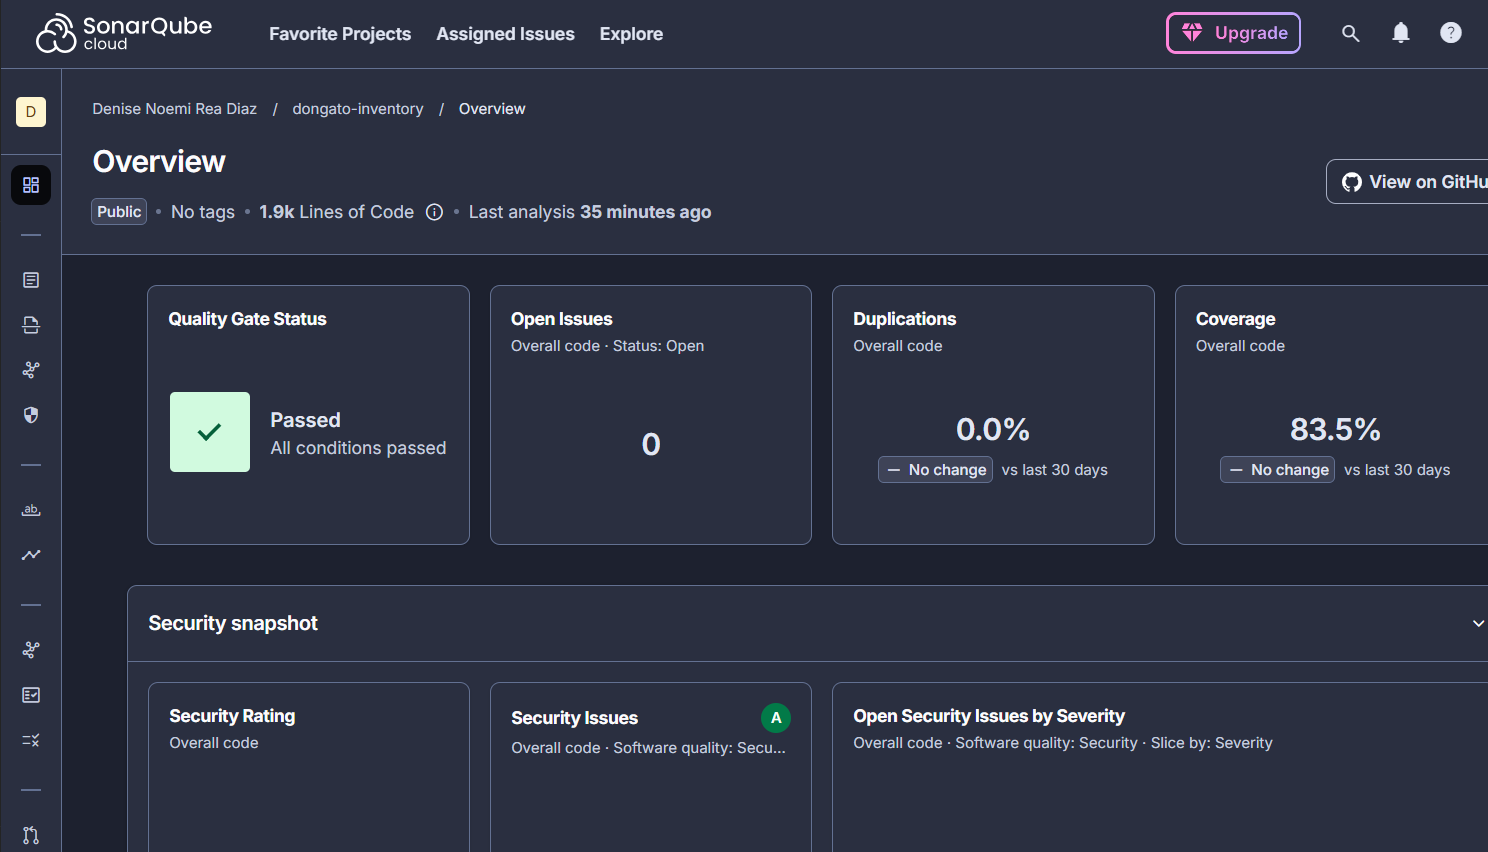
\includegraphics[width=.94\textwidth]{captura_sonarqube_quality_gate.png}
\caption{SonarCloud final: Quality Gate aprobado, 0 open issues, 0.0\% de duplicacion, 83.5\% de cobertura \textit{overall code} y Security Rating A.}
\end{figure}

\begin{figure}[H]
\centering
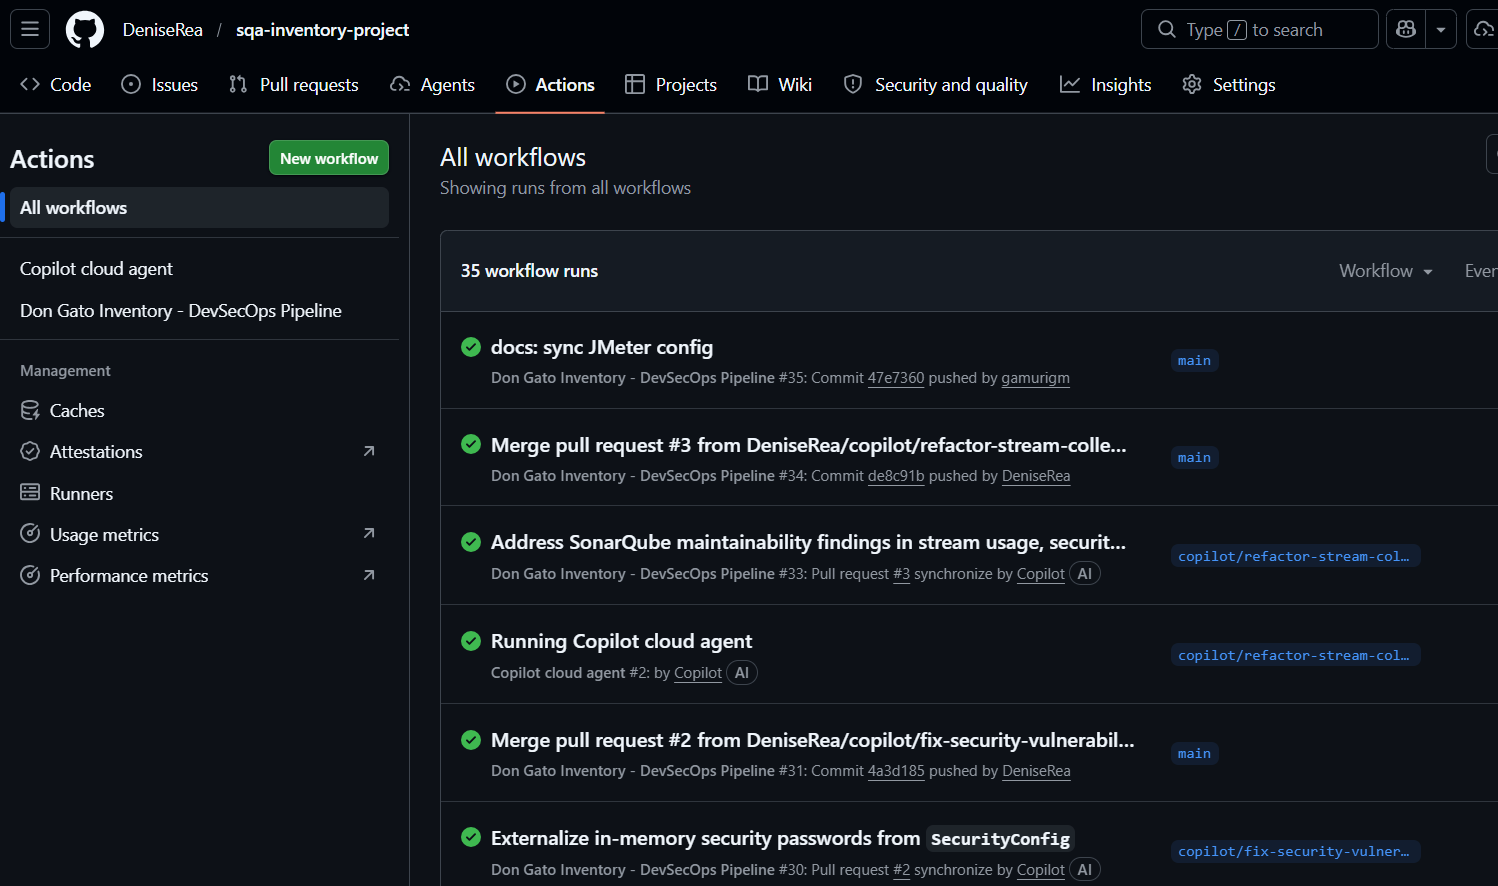
\includegraphics[width=.94\textwidth]{captura_pipeline_github_actions.png}
\caption{GitHub Actions: historial del workflow Don Gato Inventory - DevSecOps Pipeline con corridas recientes exitosas.}
\end{figure}

\begin{figure}[H]
\centering
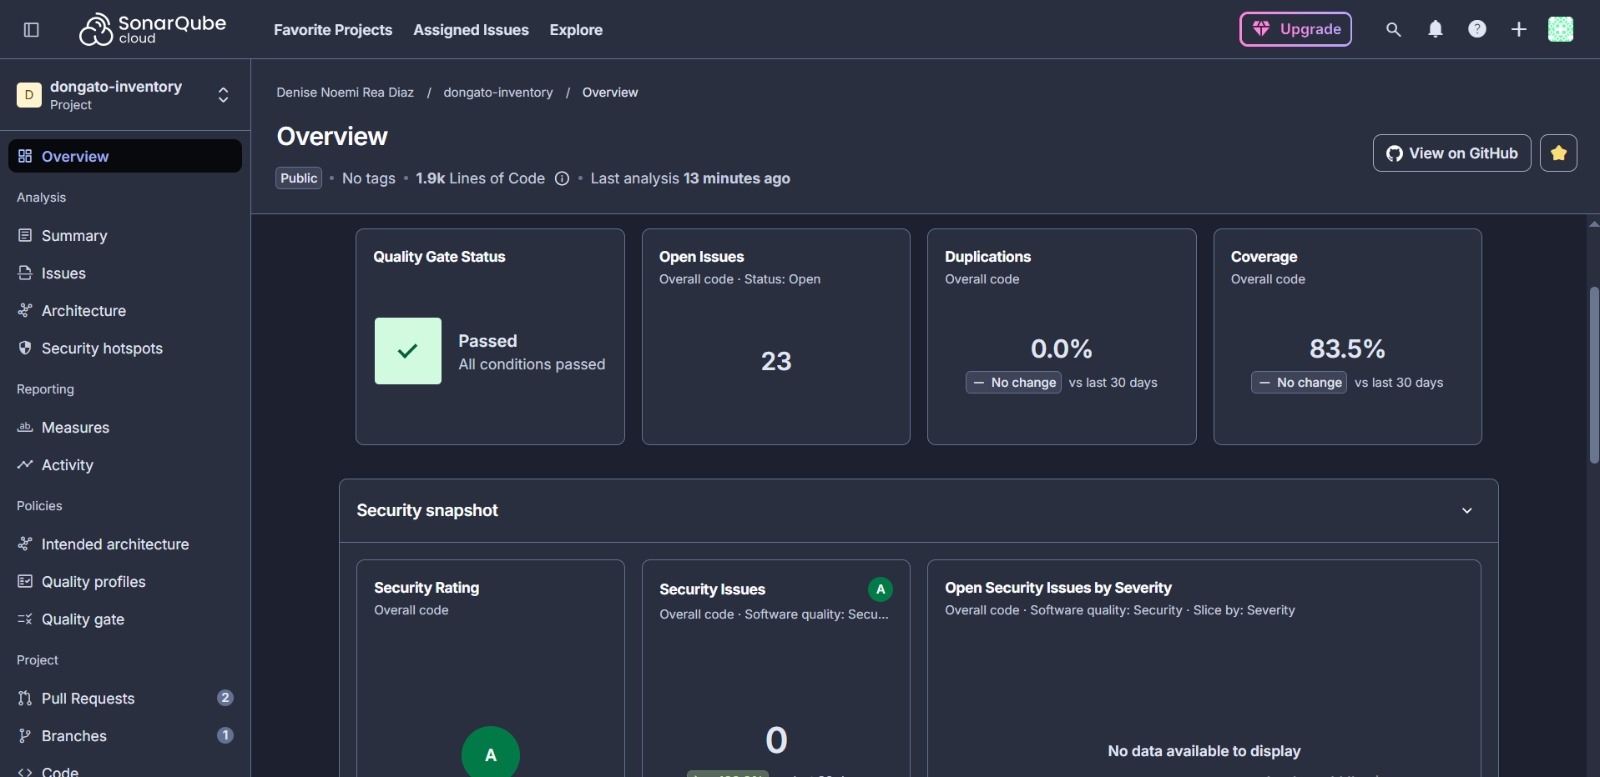
\includegraphics[width=.49\textwidth]{captura_sonarqube_before.jpeg}\hfill
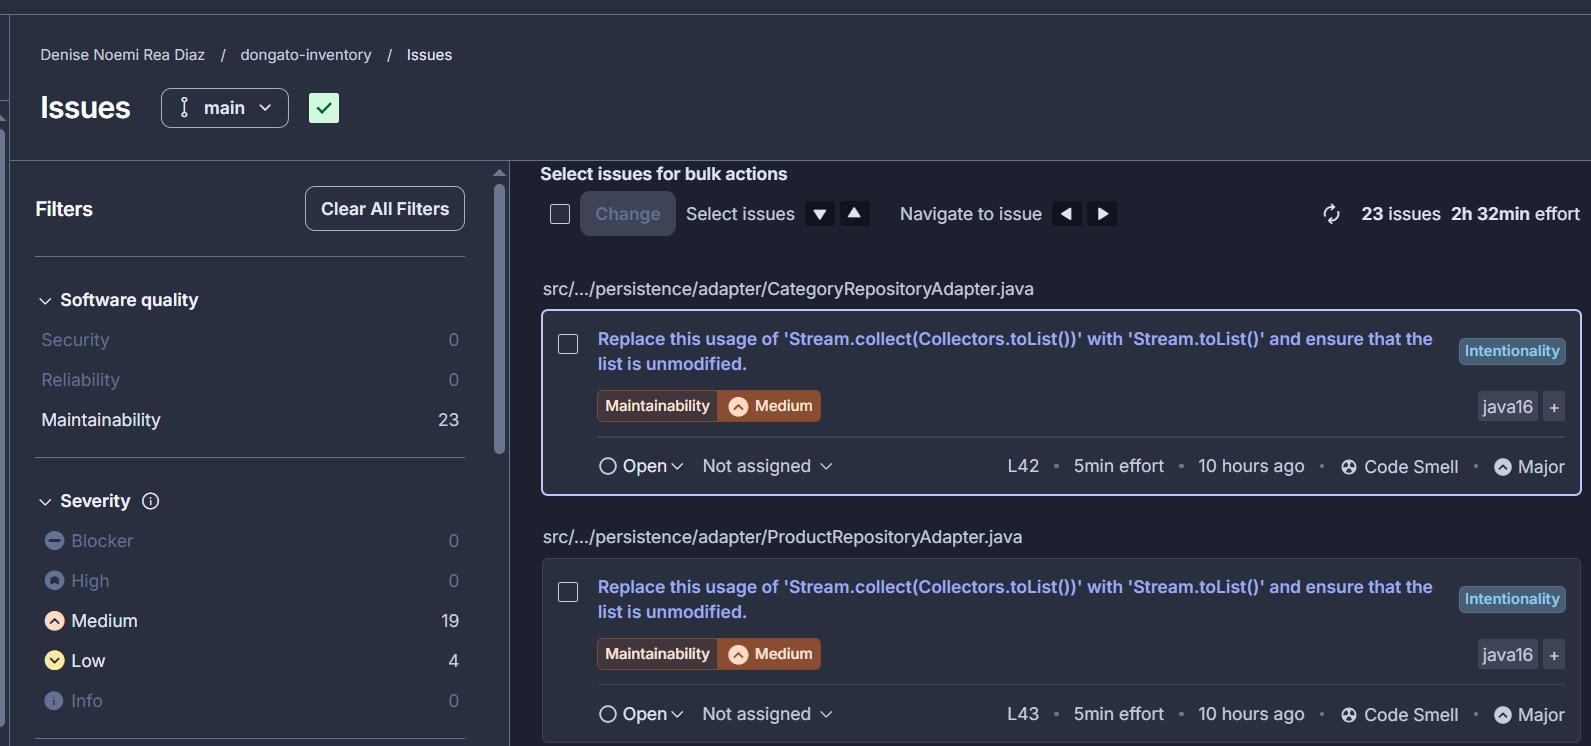
\includegraphics[width=.49\textwidth]{captura_sonarqube_issues_before.jpeg}
\caption{Estado inicial en SonarCloud: 23 issues de mantenibilidad, 19 de severidad media y 4 de severidad baja.}
\end{figure}

% -----------------------------------------------------------------------------
\section{Discusion}

\subsection{Factores McCall mas Criticos}

Los factores mas relevantes para este MVP son Integrity, Correctness, Testability y Maintainability. Integrity es prioritario porque el inventario no debe ser alterado por usuarios no autorizados. Correctness es critico porque una entrada o salida incorrecta afecta directamente el stock disponible. Testability permite evolucionar el sistema sin perder confiabilidad. Maintainability sostiene la escalabilidad del proyecto al separar responsabilidades por capas.

\begin{table}[H]
\centering
\small
\caption{Analisis de factores criticos}
\begin{tabularx}{\textwidth}{p{.20\textwidth}Yp{.28\textwidth}}
\toprule
Factor & Justificacion & Evidencia en el proyecto\\
\midrule
Integrity & Protege operaciones sensibles de inventario y administracion. & JWT, SecurityConfig y rutas protegidas.\\
Correctness & Evita inconsistencias de stock y respuestas funcionales incorrectas. & Reglas de dominio y pruebas automatizadas.\\
Testability & Reduce riesgo de regresiones durante cambios futuros. & 146 pruebas y cobertura de lineas de 90.77\%.\\
Maintainability & Permite extender el sistema sin mezclar responsabilidades. & Clean Architecture, puertos y separacion por capas.\\
Portability & Facilita reproduccion del entorno en otros equipos. & Maven Wrapper, Dockerfile y Docker Compose.\\
\bottomrule
\end{tabularx}
\end{table}

\subsection{Limitaciones Encontradas}

Aunque el MVP cumple el objetivo academico, existen limitaciones que deben considerarse en una evolucion posterior. La cobertura de ramas es menor que la cobertura de lineas, por lo que conviene fortalecer pruebas sobre caminos alternos, errores de validacion y excepciones de seguridad. Ademas, OWASP y JMeter estan incorporados como parte del flujo de calidad, pero aun deben publicarse como artefactos finales del pipeline si se exige evidencia visual independiente.

Otra limitacion es que SonarCloud y JaCoCo no reportan exactamente el mismo porcentaje de cobertura porque miden alcances distintos. Por esta razon, el informe separa la cobertura local de JaCoCo, usada para el Quality Score, de la cobertura \textit{overall code} presentada en SonarCloud. Finalmente, el MVP todavia no incluye paginacion avanzada, roles finos por perfil ni documentacion OpenAPI generada automaticamente.

\subsection{Decisiones Arquitectonicas}

La decision central fue usar Clean Architecture para proteger el dominio de detalles externos. Esta estructura permite que los casos de uso dependan de puertos y que la infraestructura implemente los adaptadores necesarios para persistencia, seguridad y comunicacion HTTP. Con ello, el proyecto mejora su mantenibilidad y conserva una base clara para agregar nuevos modulos.

La seguridad con JWT se eligio porque el frontend funciona como cliente desacoplado y necesita enviar credenciales en cada solicitud protegida mediante el encabezado \texttt{Authorization}. PostgreSQL se selecciono como base relacional principal por su uso empresarial, mientras que H2 permite ejecutar pruebas rapidas sin depender de infraestructura externa.

\subsection{Comparativa con Enfoques Alternativos}

\begin{table}[H]
\centering
\small
\caption{Comparativa de enfoques de desarrollo}
\begin{tabularx}{\textwidth}{p{.27\textwidth}Yp{.31\textwidth}}
\toprule
Alternativa & Ventaja & Riesgo frente al enfoque usado\\
\midrule
CRUD simple por capas & Menor tiempo inicial de implementacion. & Mayor acoplamiento entre controladores, entidades y repositorios.\\
MVP sin JWT & Configuracion inicial mas sencilla. & Operaciones criticas quedan expuestas o dependen de controles externos.\\
Desarrollo sin pruebas automatizadas & Avance aparente mas rapido. & Mayor probabilidad de regresiones y baja evidencia de calidad.\\
Base embebida como unica persistencia & Entorno local simple. & Menor cercania a un ambiente empresarial real.\\
Clean Architecture + DevSecOps & Mayor trazabilidad y escalabilidad. & Requiere mas disciplina tecnica y configuracion inicial.\\
\bottomrule
\end{tabularx}
\end{table}

El enfoque seleccionado exige mas estructura al inicio, pero ofrece mejor soporte para evolucionar el sistema, justificar la calidad con metricas y sostener futuras integraciones.

% -----------------------------------------------------------------------------
\section{Conclusiones}

\subsection{Lecciones Aprendidas sobre Calidad Medible}

El proyecto demuestra que la calidad debe definirse desde el inicio mediante criterios verificables. La cobertura, los resultados de pruebas, la seguridad por rutas y el Quality Score permiten transformar conceptos generales de calidad en evidencia concreta. Tambien se confirma que Clean Architecture facilita la trazabilidad entre requisitos, reglas de negocio y pruebas.

El Modelo de McCall resulto util para explicar por que se tomaron determinadas decisiones tecnicas. La seguridad JWT se relaciona con Integrity, las pruebas automatizadas con Testability y Reliability, la separacion de capas con Maintainability y la API versionada con Interoperability.

\subsection{Recomendaciones para Escalar el Framework}

Para fortalecer el proyecto se recomienda consolidar SonarCloud dentro de GitHub Actions como gate obligatorio, ejecutar \texttt{mvnw verify} antes de cada merge, publicar artifacts de JaCoCo, OWASP y JMeter en cada corrida de CI, e incorporar OpenAPI/Swagger como documentacion viva de endpoints.

Tambien se recomienda implementar roles y permisos mas finos para administrador, cajero y consulta; introducir Testcontainers para validar persistencia con PostgreSQL real; y extender el Quality Scoring Engine para leer reportes generados automaticamente, evitando calculos manuales.

\subsection{Trabajo Futuro}

Como trabajo futuro se plantea complementar McCall con ISO 25010, incorporar IA en testing para generar casos borde y datos sinteticos, medir p95/p99 de latencia en un ambiente controlado, agregar cache selectivo para consultas publicas de productos e integrar monitoreo continuo de calidad en el pipeline.

En conclusion, Don Gato Inventory entrega una API REST educativa con estructura empresarial: seguridad JWT, Clean Architecture, pruebas automatizadas, cobertura superior al umbral, trazabilidad PDCA, evaluacion por McCall y una ruta clara de mejora continua mediante DevSecOps.

\end{document}
